\chapter{\textbf{Аналитический раздел}}
\hfill

Целью работы является создание максимально приближенной модели взрыва большого числа частиц. Объекты в сцене представлены в виде твердых частиц, которые приводятся в движение различными силами.  

\section{\textbf{Анализ предметной области }}

\textbf{Система частиц} --- широко используемый в компьютерной графике метод представления объектов, не имеющих четких геометрических границ. Облака, туманности, дым, взрыв, снег --- все эти объекты моделируются с помощью систем частиц. Системы частиц --- множество частиц с индивидуальными свойствами, а не поверхность с текстурой. При таком подходе возможно изменять внешний вид каждой отдельной частицы с течением времени и, таким образом, создавать визуализации, которые реалистично отображают огонь, дым, воду, взрывы и даже волосы и мех. Они также используются для представления неестественных явлений.  \cite{definition}

Уже в начале 1980-х годов Уильям Т. Ривз использовал системы частиц для моделирования огня, поглощающего планету, в фильме «Звёздный путь II: Гнев Хана». Ривз считается изобретателем систем частиц, и в 1983 году он опубликовал статью, объясняющую, как это было сделано. Ривз продолжил развивать эту идею и с тех пор внёс большой вклад в данную область. Разработка продолжалась, и сегодня большинство игровых движков содержат систему частиц. \cite{particlesystems}

Эта техника имеет много полезных приложений, будь то большие взрывы, пыль, пожары или большие толпы людей, спецэффекты необходимы во многих фильмах, анимациях, съемках или компьютерных играх. Фильмы, показывающие массивные взрывы и разрушенные здания, могут имитировать эти эффекты, а не создавать их по-настоящему. В этой работе стоит задача визуализации взрыва большого числа частиц, при столкновении с телом.
	
Визуализация взрыва частиц может быть описана по-разному в зависимости от источника силы, порождающий взрыв. В данной работе, источником является шарообразное тело, врезающееся в систему более мелких частиц.
	
На сцене располагается неподвижная, в начальный момент, группа частиц, расположенных вместе, шарообразное подвижное тело, точечный источник света.
	
В начальный момент времени, есть возможность скорректировать положение системы, поменять расположение камеры.
	
После нажатия на кнопку, произойдёт симуляция.

На рисунке \ref{img:idef0} изображена \textbf{функциональная модель}, отображающая структуру и функции системы. 

\begin{figure}[H]
	\centering
	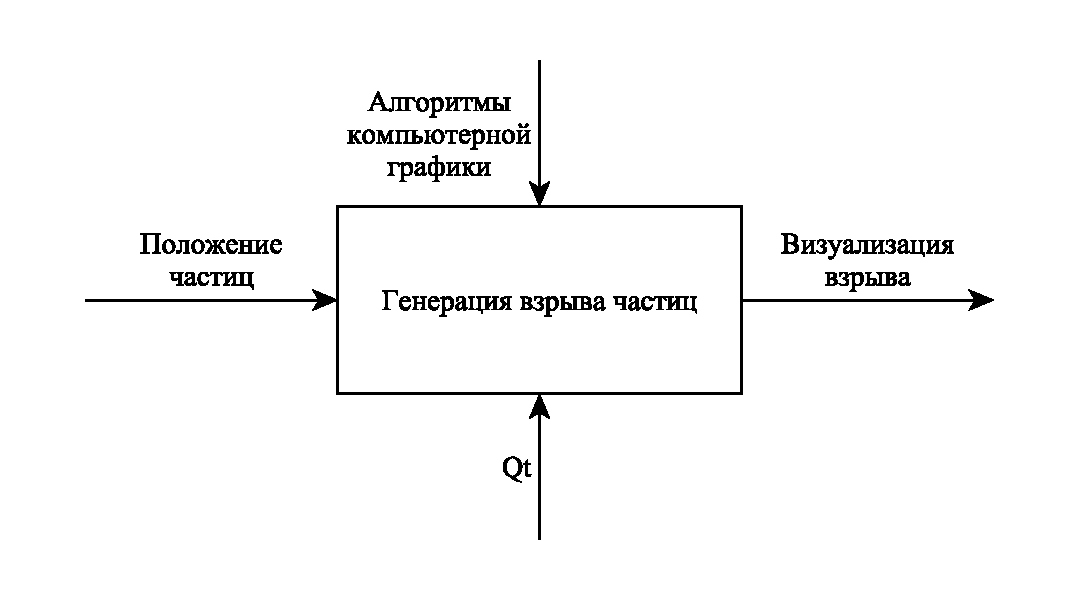
\includegraphics[scale=0.9]{idef0}
	\caption{Функциональная модель процесса визуализации взрыва частиц. }
	\label{img:idef0}
\end{figure}

На вход принимаются частицы с различными параметрами (положение, масса, размер) и положение шарообразного врезающегося тела, с идентичными параметрами. На выходе получаем визуализацию взрыва мелких частиц при столкновении с телом. 

В рамках данного исследования существует возможность, менять параметры частиц. 

\section{\textbf{Обзор и анализ существующих решений, обоснование необходимости разработки}}

\textbf{В настоящее время при 3D моделировании объекты создают в основном только двумя способами.} \cite{3dgraphic}
\begin{enumerate}
	\item[1. ] Либо с помощью плоских полигонов — тем самым будет создана полая модель без внутреннего наполнения. 
	\item[2. ] Либо с помощью частиц, которые полностью заполняют внутренности модели, где каждая частица представляется как материальная точка с дополнительными атрибутами, такими как скорость, цвет, ориентация в пространстве, угловая скорость и т. п.
\end{enumerate}

Ввиду того, что полигональные модели пусты по своей природе, очень трудно моделировать их поведение в 3D мире, как, например, всплески воды. Если же воду моделировать через систему частиц, то всё становится гораздо проще, так как вся вода от поверхности океана и до дна состоит из атомов, которые можно рассматривать, как набор отдельных частиц.

\textbf{Далее рассматриваются алгоритмы удаления невидимых поверхностей. } \cite{deletenovisible}

\begin{enumerate}
	\item[1. ] Алгоритм, использующий z-буфер. 
	\item[2. ] Алгоритм разбиения области Варнока. 
	\item[3. ] Метод трассировки лучей. 
\end{enumerate}

\textbf{Алгоритм удаления поверхностей с Z-буфером }

Алгоритм предложен Эдом Кэтмулом и представляет собой обобщение буфера кадра. Обычный буфер кадра хранит коды цвета для каждого пиксела в пространстве изображения. Идея алгоритма состоит в том, чтобы для каждого пиксела дополнительно хранить еще и координату Z или глубину. При занесении очередного пиксела в буфер кадра значение его Z-координаты сравнивается с Z-координатой пиксела, который уже находится в буфере. Если Z-координата нового пиксела больше, чем координата старого, т.е. он ближе к наблюдателю, то атрибуты нового пиксела и его Z-координата заносятся в буфер, если нет, то ни чего не делается. Таким образом, после выполнения этих операций в каждой точке экрана будет находиться пиксель, соответствующий грани, находящейся ближе всего к картинной плоскости в данной точке.

Этот алгоритм наиболее простой из всех алгоритмов удаления невидимых поверхностей, но требует большого объема памяти. Время работы алгоритма не зависит от сложности сцены. Многоугольники, составляющие сцену, могут обрабатываться в произвольном порядке. 

Основной недостаток алгоритма с Z-буфером - дополнительные затраты памяти. Другие недостатки алгоритма с Z-буфером заключаются в том, что так как пикселы в буфер заносятся в произвольном порядке, то возникают трудности с реализацией эффектов прозрачности или просвечивания и устранения лестничного эффекта. 

\textbf{Алгоритм разбиения области Варнока }

Алгоритм работает в пространстве изображения и анализирует область на экране дисплея (окно) на наличие в нём видимых элементов. Если в окне нет изображения, то оно просто закрашивается фоном. Если же в окне имеется элемент, то проверяется достаточно ли он прост для визуализации. Если объект сложный, то окно разбивается на более мелкие, для каждого из которых выполняется тест на отсутствие и/или простоту изображения. Рекурсивный процесс разбиения может продолжаться до тех пор пока не будет достигнут предел разрешения экрана (1 пиксель).

Можно выделить 4 случая взаимного расположения окна и многоугольника (рис. \ref{img:varnok}):
\begin{enumerate}
	\item многоугольник целиком вне окна;
	\item многоугольник целиком внутри окна;
	\item многоугольник пересекает окно;
	\item многоугольник охватывает окно.
\end{enumerate}

\begin{figure}[H]
	\centering
	\includegraphics[scale=0.7]{varnok}
	\caption{Соотношения между окном экрана (сплошная рамка) и многоугольником (штриховая рамка). }
	\label{img:varnok}
\end{figure}

В четырех случаях можно сразу принять решение о правилах закраски области экрана:
\begin{enumerate}
	\item все многоугольники сцены - внешние по отношению к окну. В этом случае окно закрашивается фоном;
	\item имеется всего один внутренний или пересекающий многоугольник. В этом случае все окно закрашивается фоном и затем часть окна, соответствующая внутреннему или пересекающему окну закрашивается цветом многоугольника;
	\item имеется единственный охватывающий многоугольник. В этом случае окно закрашивается его цветом;
	\item имеется несколько различных многоугольников и хотя бы один из них охватывающий. Если при этом охватывающий многоугольник расположен ближе остальных к наблюдателю, то окно закрашивается его цветом.
\end{enumerate}
В любых других случаях процесс разбиения окна продолжается.

Алгоритм работает с многоугольниками. 

\textbf{Алгоритм трассировки лучей }

Суть метода заключается в том, что для каждой точки на проектируемой плоскости строится луч, начало которого совпадает с положением наблюдателя, а угол луча по отношению к направлению наблюдения определяется характеристиками наблюдателя (максимальный угол зрения относительно горизонтальной и вертикальной плоскостей) и точкой плоскости проецирования (картинная плоскость), для которой строится луч. 

После построения луча определяется его пересечение со всеми гранями, из которых состоит сцена и выбирается та грань, расстояние от которой до наблюдателя минимально.

 Далее в данной точке картинной плоскости рисуется пиксель цветом, определяемым в точке пересечения луча и выбранной грани. 
 
 Этот метод является довольно простым и позволяет совместить определение видимости с расчётом цвета соответствующего пикселя. Ещё одним преимуществом метода является то, что сцена может состоять не из треугольников, а быть задана набором геометрических примитивов (например, поверхностями второго порядка). В этом случае пересечение луча с геометрическим примитивом вычисляется аналитически (точное решение задачи построения геометрического примитива), в отличие от разбивания произвольного геометрического примитива (например, сферы) на треугольники и решения более простой задачи пересечения луча с треугольником. 
 
 Могут генерироваться новые лучи внутри сцены для корректного отображения отражений, преломлений, затенений --- алгоритм обратной трассировки лучей более эффективен.
 
Может быть модифицирован для отображения общего освещения сцены. 

Тем не менее для реализации метода требуется довольно большое количество вычислений и, следовательно, большие временные затраты. 


\textbf{Актуальность темы} исследования обусловлена тем, что за последние несколько лет технологии компьютерной симуляции совершили огромный скачок в развитии и расширении сфер применения. Если раньше эти технологии в основном применялись в военной промышленности и компьютерных играх, то сейчас компьютерная симуляция проникает практически во все сферы деятельности человека: медицину, образование, архитектуру, рекламу и прочее. Эта технология имеет огромный потенциал и поэтому она так активно развивается.

\section{\textbf{Выбор, обоснование метода моделирования и алгоритма}}

На основании предложенных методов моделирования, в данной работе будет использоваться система частиц (а именно сфер). 

Для удаления невидимых поверхностей будет реализован алгоритм обратной трассировки лучей, несмотря на вычислительную сложность, алгоритм предоставляет возможность работать непосредственно со сферическими поверхностями и отображать освещение. 

\section{\textbf{Вывод}}

В данной работе ставится задача визуализации взрыва системы частиц при столкновении с шарообразным телом, используя алгоритм обратной трассировки, как наиболее оптимальный для поставленной задачи. 

На сцене располагается неподвижная, в начальный момент, группа частиц, расположенных вместе, шарообразное подвижное тело, точечный источник света.
	
В начальный момент времени, есть возможность скорректировать размеры тела, поменять расположение камеры.
	
После нажатия на кнопку, произойдёт симуляция.